%%% -------------------------------------------------------------------- %%%
%%% -----------------------------Приложения----------------------------- %%%
%%% -------------------------------------------------------------------- %%%

%%% ----------------------------Приложение А---------------------------- %%%
\ESKDappendix{обязательное}{Подключение источника питания к плате \DocProductShortTitle~ через адаптер}

\label{appendix:power_adapter}

\begin{figure}[!h]
\center{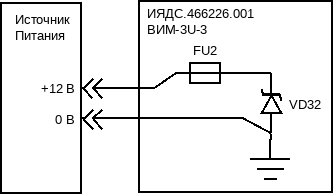
\includegraphics[scale=0.8]{vim_power_adapter_connection_sch.png}} 
\caption{Схема подключения источника питания к плате \DocProductShortTitle~}
\label{ris:vim_power_connection}
\end{figure}

\begin{figure}[!h]
\center{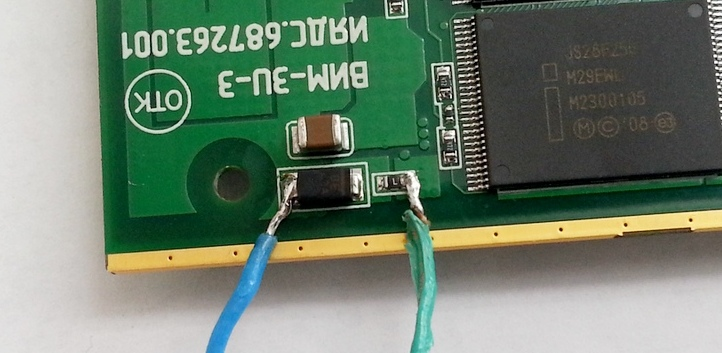
\includegraphics[width=1\linewidth]{vim_vcc12_adapter_solder_foto.jpg}} 
\caption{Фотография места пайки при подключении источника питания к плате \DocProductShortTitle~}
\label{ris:vim_vcc12_adapter_solder_foto}
\end{figure}

%%%Технологическая перемычка нужна долько для программирования ПЛИС вне стенда. Исключаем (?временно) этот пункт
%\begin{figure}[!h]
%\center{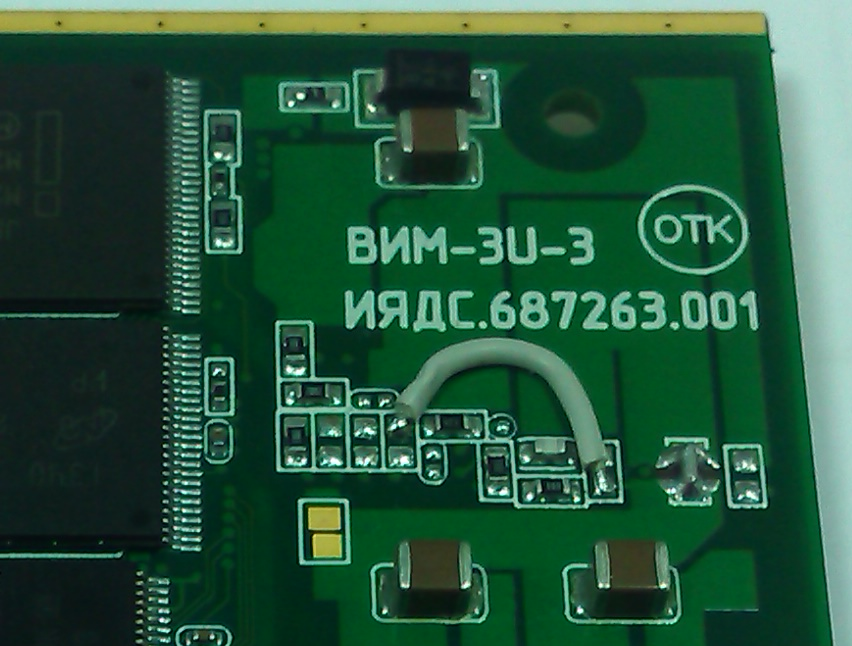
\includegraphics[width=1\linewidth]{vim_3v3aux_tech_jumper_foto.jpg}}
%\caption{Фотография места установки технологической перемычки на плате \DocProductShortTitle~}
%\label{ris:vim_3v3aux_tech_jumper_foto}
%\end{figure}

%%% ----------------------------Приложение Б---------------------------- %%%
\ESKDappendix{обязательное}{Установка перемычек по цепям питания на плате \DocProductShortTitle~}
\label{appendix:power_jumpers}

\begin{figure}[!h]
\center{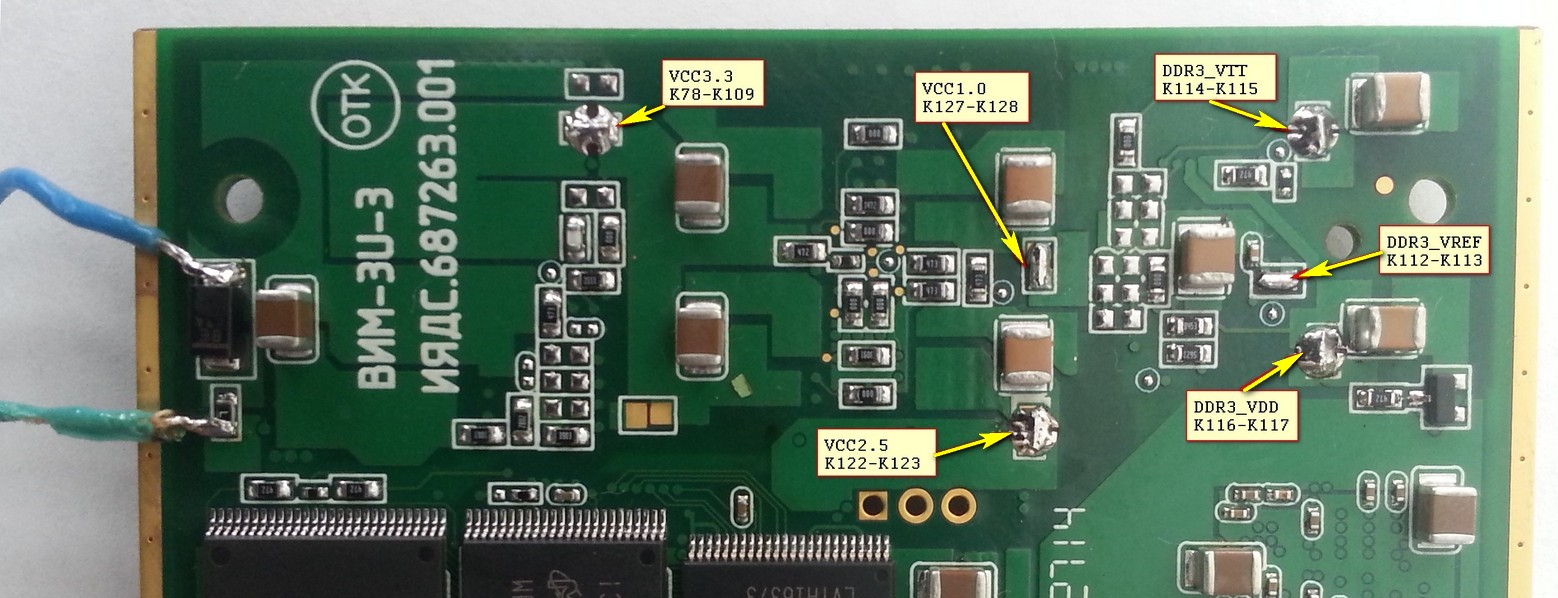
\includegraphics[width=1\linewidth]{vim_power_jumper_foto.jpg}} 
\caption{Фотография установленных перемычек по цепям питания на плате \DocProductShortTitle~}
\label{ris:vim_power_jumper_foto}
\end{figure}

%%% --------------------------------END--------------------------------- %%%


